\subsection{Комплексный квадрат}
Рассмотрим комплексную функцию  $f_5(t)$:

\begin{equation}
    Re f_5(t) = \begin{cases}
        3, & t \in [-\frac{1}{2}, \frac{1}{2})\\[0.75pt]
        6 - 6t, & t \in [\frac{1}{2}, \frac{3}{2})\\[0.75pt]
        -3, & t \in [\frac{3}{2}, \frac{5}{2})\\[0.75pt]
        -18 + 6t, & t \in [\frac{5}{2}, \frac{7}{2})\\[0.75pt]
    \end{cases} 
    ~~~~~
    Im f_5(t) = \begin{cases}
        6t, & t \in [-\frac{1}{2}, \frac{1}{2})\\[0.75pt]
        3, & t \in [\frac{1}{2}, \frac{3}{2})\\[0.75pt]
        12 - 6t, & t \in [\frac{3}{2}, \frac{5}{2})\\[0.75pt]
        -3, & t \in [\frac{5}{2}, \frac{7}{2})\\[0.75pt]
    \end{cases}
\label{eq:complex_func}
\end{equation}

График этой функции представлен на рисунке~\ref{fig:complex_func}.

\begin{figure}[ht!]
    \centering
    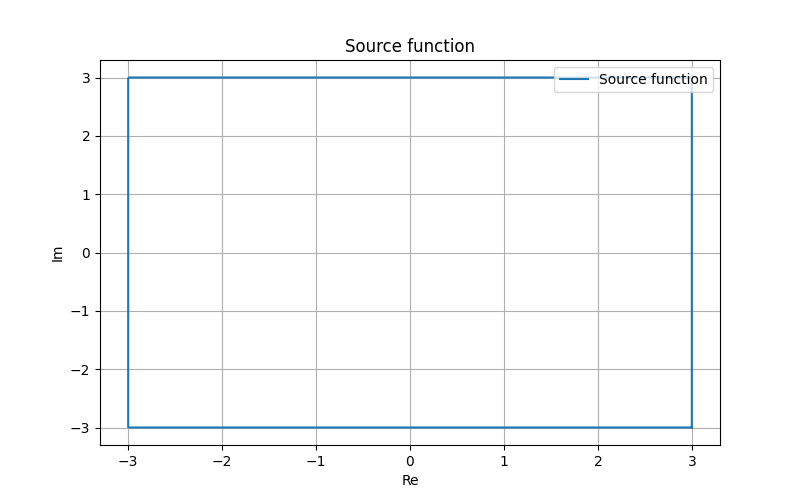
\includegraphics[width=\textwidth]{./media/plots/func_5.png}
    \caption{График комплексной функции $f_5(t)$}
    \label{fig:complex_func}
\end{figure}

\subsubsection{Вычисление коэффициентов Фурье}
Найдем коэффициенты ряда Фурье для этой функции в соответствии с формулой~\ref{eq:fourier_coefficients_exp}.

\begin{multline}
    c_n = \frac{1}{4}\int\limits_{-0.5}^{3.5} f_5(t) e^{-i \frac{\pi nt}{2}} dt = \frac{1}{4} ( \int\limits_{-0.5}^{0.5} (3 + 6ti)e^{-i \frac{\pi nt}{2}} dt + \int\limits_{0.5}^{1.5} (6 - 6t + 3i)e^{-i \frac{\pi nt}{2}} dt \\
    + \int\limits_{1.5}^{2.5}(-3 + (12 - 6t)i) e^{-i \frac{\pi nt}{2}} dt + \int\limits_{2.5}^{3.5}(-18 + 6t - 3i) e^{-i \frac{\pi nt}{2}} dt )
\end{multline}

\subsubsection{Вычисление коэффициентов Фурье с помощью программы}

\begin{lstlisting}[style=python_white, caption=Вычисление коэффициентов Фурье, label=lst:func_5]
R = 3
T = 4

def func(t):
    real = -1
    if -T/8 <= t < T/8:
        real = R
    if T/8 <= t < 3 * T / 8:
        real = 2 * R - 8 * R * t / T 
    if 3 * T / 8 <= t < 5 * T / 8:
        real = -R
    if 5 * T / 8 <= t <= 7 * T / 8:
        real = -6 * R + 8 * R * t / T

    imag = -1
    if -T/8 <= t < T/8:
        imag = 8 * R * t / T
    if T/8 <= t < 3 * T / 8:
        imag = R
    if 3 * T / 8 <= t < 5 * T / 8:
        imag = 4 * R - 8 * R * t / T
    if 5 * T / 8 <= t <= 7 * T / 8:
        imag = -R

    return real + 1j * imag

func = np.vectorize(func)
c = fourier_exp(func, -T/8, T, 3)
print_fourier_exp_coefficients(c)
\end{lstlisting}

В результате выполнения программы (\ref{lst:func_5}) получим следующие значения (см. таблицу~\ref{tab:func_5_exp}).

\begin{table}[h!]
    \centering
    \begin{tabular}{|c|c|}
        \hline
        $n$ & $c_n$ \\
        \hline
        -3 & -0.38253+0.00000i \\
        -2 & -0.00030-0.00030i \\
        -1 & -0.00000-0.00042i \\
        0 & 0.00030-0.00030i \\
        1 & 3.43938+0.00000i \\
        2 & 0.00030+0.00030i \\
        3 & -0.00000+0.00042i \\
        \hline
    \end{tabular}
    \caption{Коэффициенты Фурье для функции $f_5(t)$ }
    \label{tab:func_5_exp}
\end{table}

\subsubsection{Построение графиков частичных сумм ряда Фурье}
В качество значений $N$ выберем $N = 1, 2, 3, 5, 10$. Для каждого значения $N$ вычислим частичную сумму ряда Фурье и построим график (см. рис.~\ref{fig:func_5_plot}).

\begin{lstlisting}[style=python_white, caption=Построение графиков частичных сумм ряда Фурье, label=lst:func_1_plot]
    calc_and_plot_parametric(func, -T/8, T, [1, 2, 3, 5, 10], './media/plots/func_5')
\end{lstlisting}

% plot with partial sums
\begin{figure}[ht!]
    \centering
    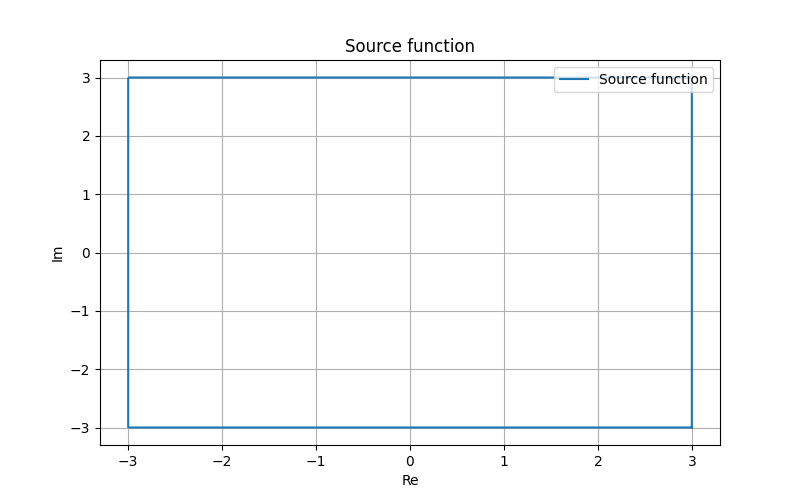
\includegraphics[width=0.49\textwidth]{media/plots/func_5.png}
    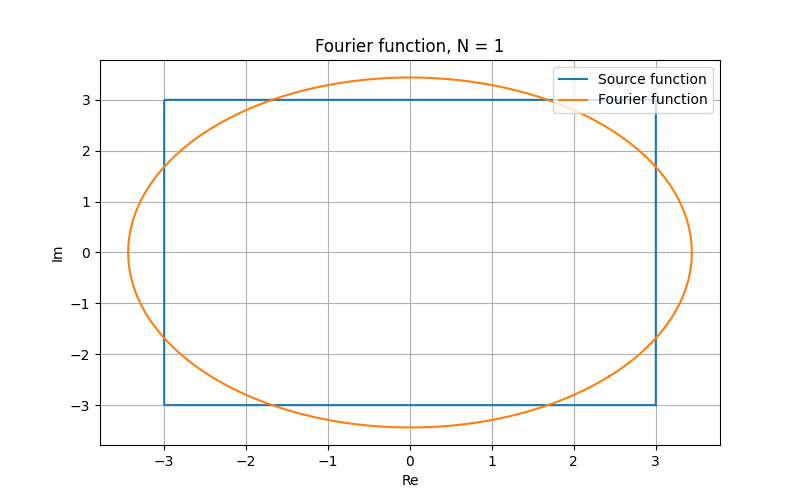
\includegraphics[width=0.49\textwidth]{media/plots/func_5_N_1.png}
    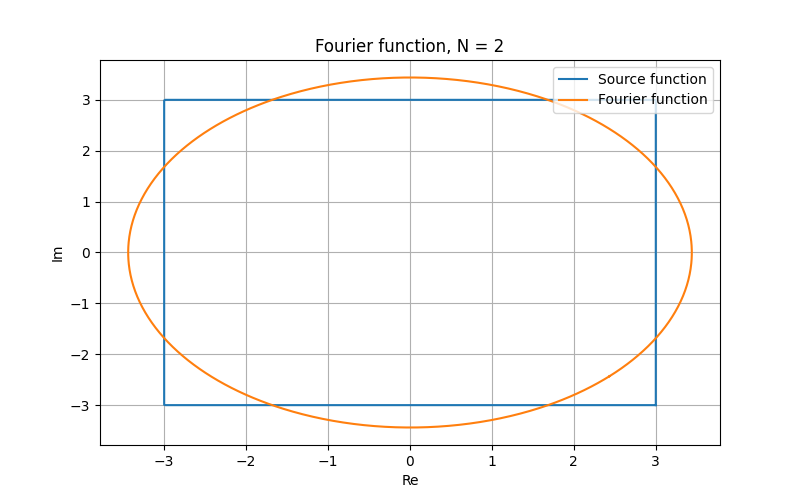
\includegraphics[width=0.49\textwidth]{media/plots/func_5_N_2.png}
    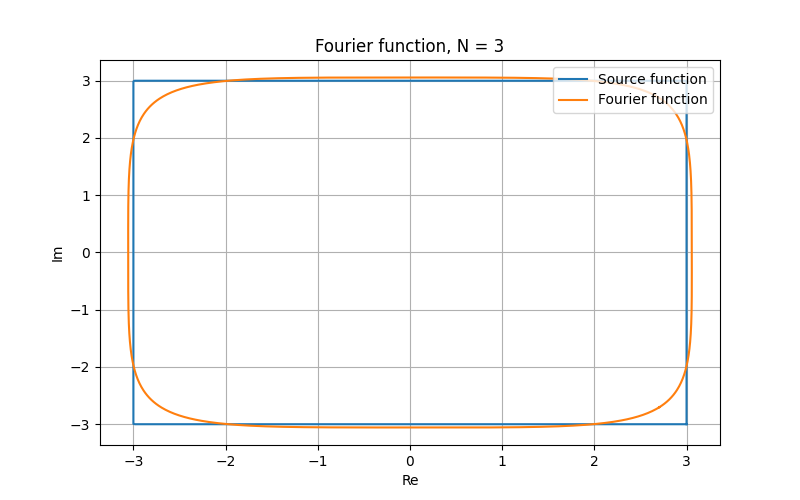
\includegraphics[width=0.49\textwidth]{media/plots/func_5_N_3.png}
    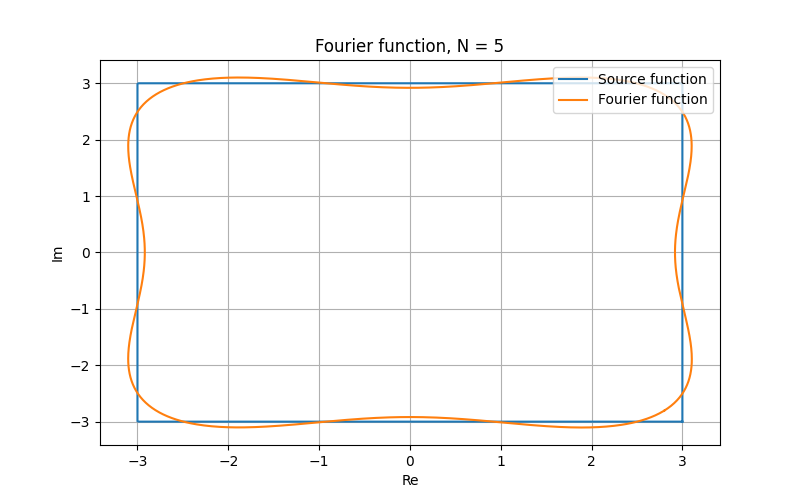
\includegraphics[width=0.49\textwidth]{media/plots/func_5_N_5.png}
    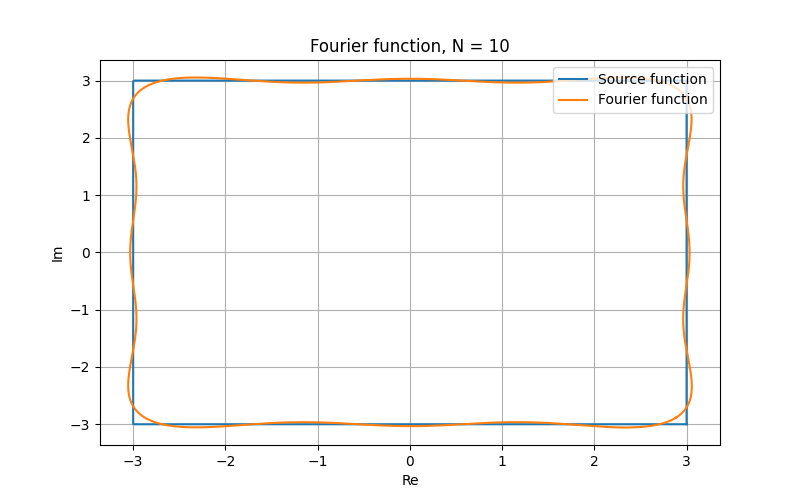
\includegraphics[width=0.49\textwidth]{media/plots/func_5_N_10.png}
    \caption{Параметрический график частичных сумм ряда Фурье для функции $f_5(t)$}
    \label{fig:func_5_plot}
\end{figure}

Видим, что как и в случае вещественных функций, при увеличении значения $N$ график частичной суммы ряда Фурье все точнее приближает исходную функцию. 
При значениях $N = 1, 2$ график частичной суммы ряда Фурье представляет из себя эллипс, при $N = 3$ -- уже похож на исходную функцию.
При значениях $N = 10$ график частичной суммы ряда Фурье довольно точно повторяет исходную функцию.

\subsection{Графики вещественной и комплексной части отдельно}

Рассмотрим графики $Re~f_5(t)$ и $Im~f_5(t)$ (см. рис.~\ref{fig:func_5_re_im}) и графики $Re~G_n(t)$ и $Im~G_n(t)$  для функции $f_5(t)$ (см. рис.~\ref{fig:func_5_fourier_re_im_N_1}~-~\ref{fig:func_5_fourier_re_im_N_10}).

\begin{figure}[ht!]
    \centering
    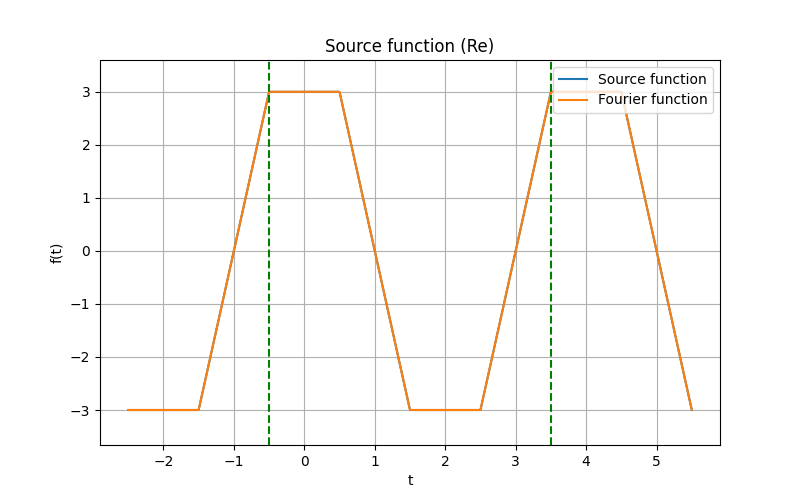
\includegraphics[width=0.49\textwidth]{media/plots/func_5_real.png}
    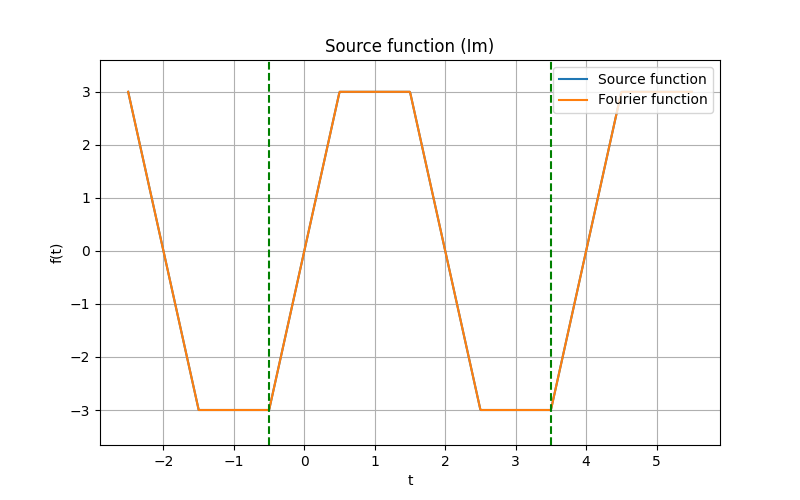
\includegraphics[width=0.49\textwidth]{media/plots/func_5_imag.png}
    \caption{График  $f_5(t)$ (действительная и мнимая часть)}
    \label{fig:func_5_re_im}
\end{figure}


\begin{figure}[ht!]
    \centering
    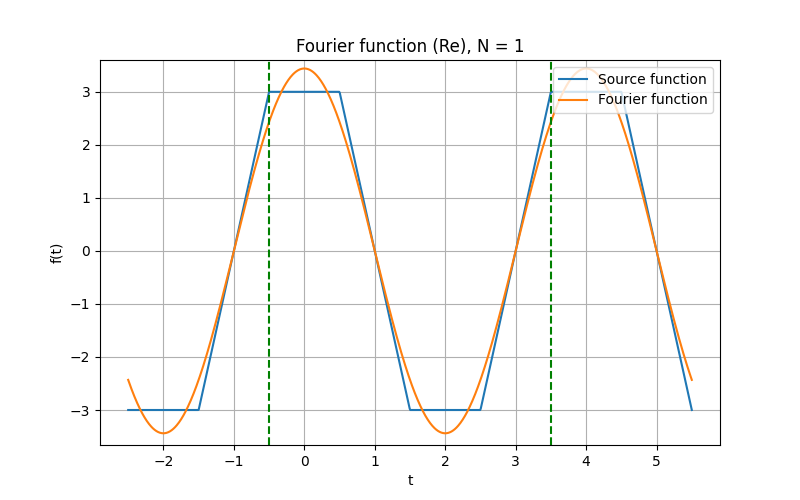
\includegraphics[width=0.49\textwidth]{media/plots/func_5_real_N_1.png}
    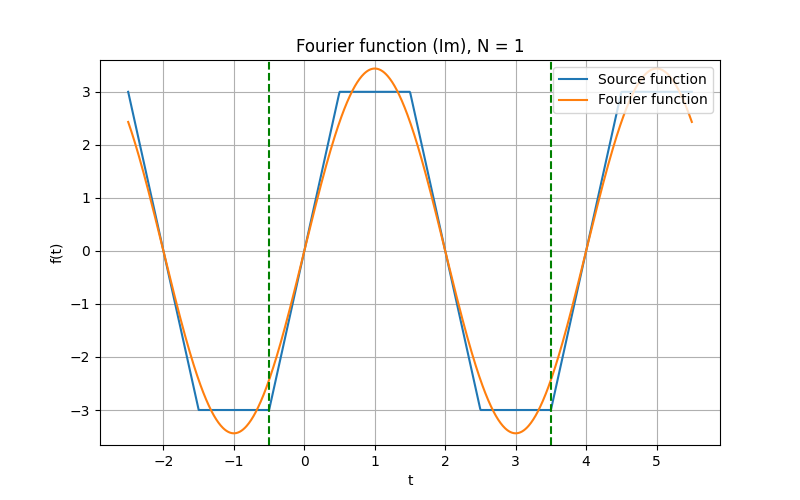
\includegraphics[width=0.49\textwidth]{media/plots/func_5_imag_N_1.png}
    \caption{График частичных сумм ряда Фурье для функции $f_5(t)$ ($N = 1$) (действительная и мнимая часть)}
    \label{fig:func_5_fourier_re_im_N_1}
\end{figure}

\begin{figure}[ht!]
    \centering
    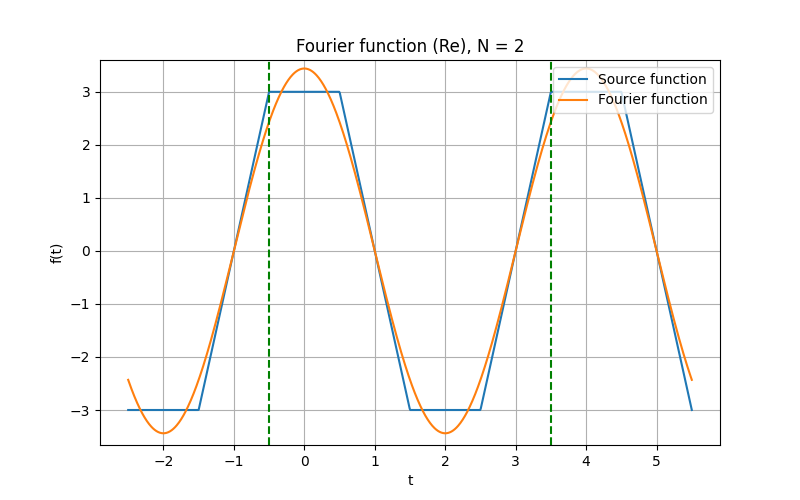
\includegraphics[width=0.49\textwidth]{media/plots/func_5_real_N_2.png}
    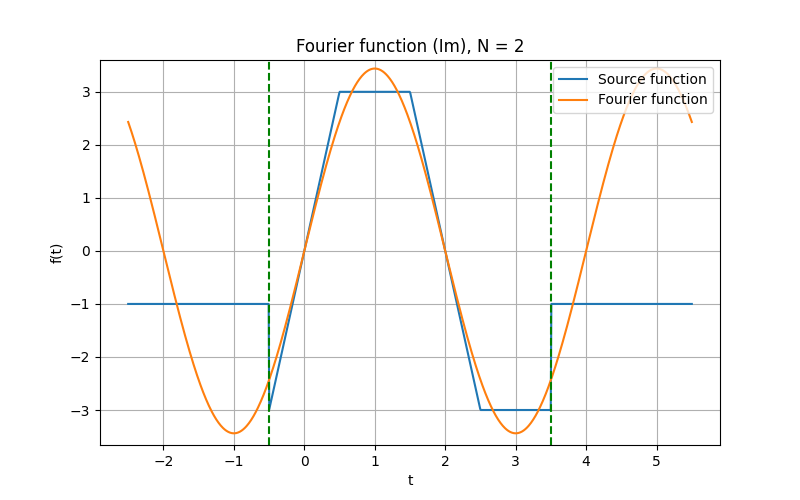
\includegraphics[width=0.49\textwidth]{media/plots/func_5_imag_N_2.png}
    \caption{График частичных сумм ряда Фурье для функции $f_5(t)$ ($N = 2$) (действительная и мнимая часть)}
    \label{fig:func_5_fourier_re_im_N_2}
\end{figure}

\begin{figure}[ht!]
    \centering
    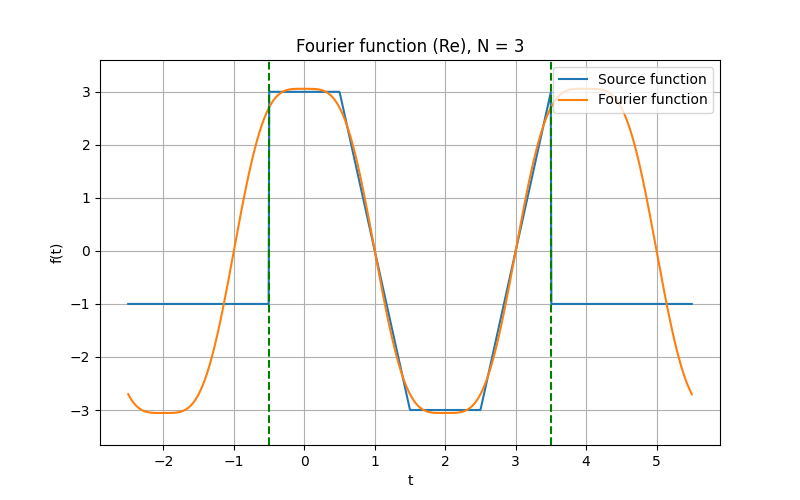
\includegraphics[width=0.49\textwidth]{media/plots/func_5_real_N_3.png}
    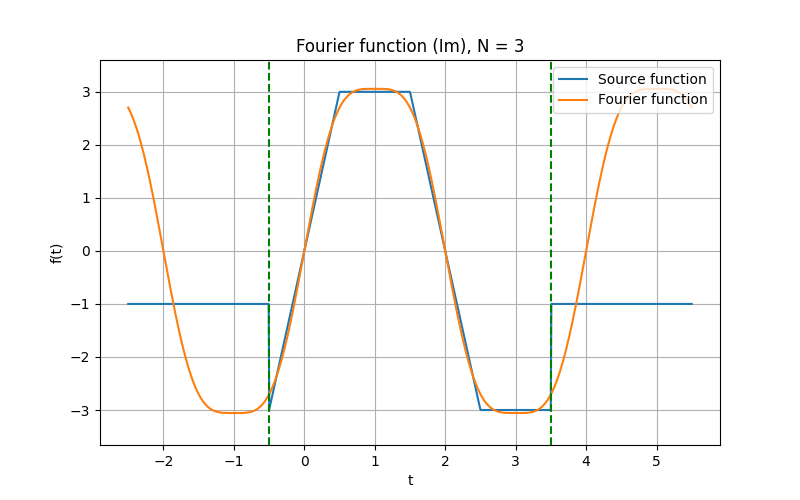
\includegraphics[width=0.49\textwidth]{media/plots/func_5_imag_N_3.png}
    \caption{График частичных сумм ряда Фурье для функции $f_5(t)$ ($N = 3$) (действительная и мнимая часть)}
    \label{fig:func_5_fourier_re_im_N_3}
\end{figure}


\begin{figure}[ht!]
    \centering
    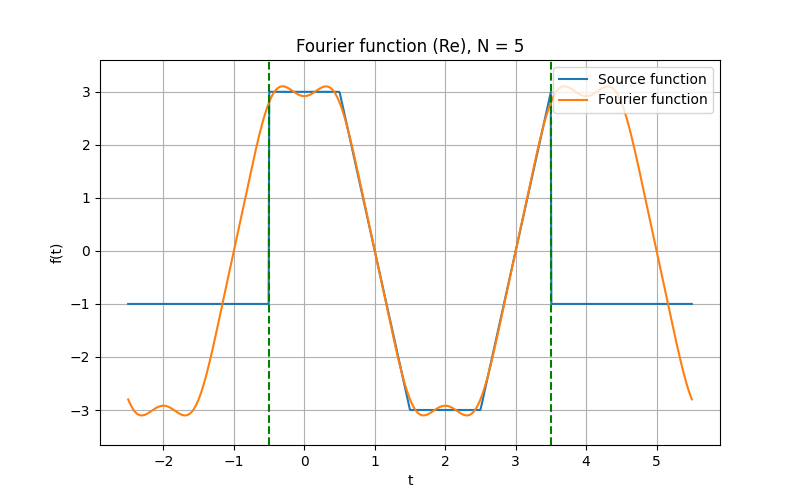
\includegraphics[width=0.49\textwidth]{media/plots/func_5_real_N_5.png}
    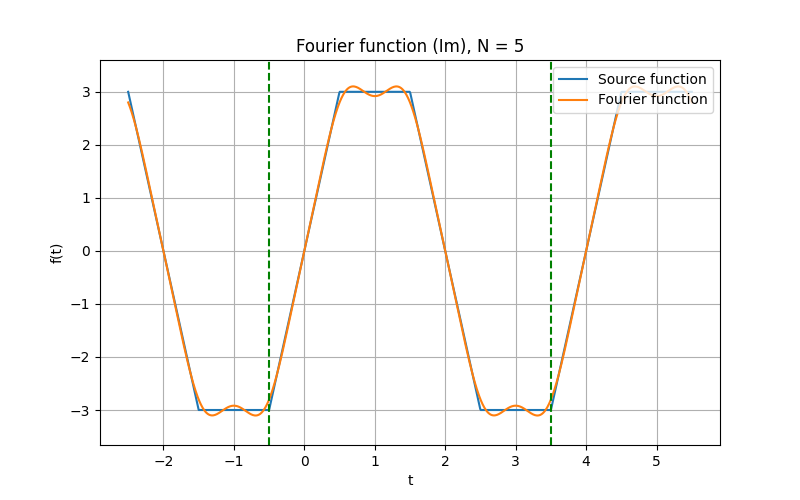
\includegraphics[width=0.49\textwidth]{media/plots/func_5_imag_N_5.png}
    \caption{График частичных сумм ряда Фурье для функции $f_5(t)$ ($N = 5$) (действительная и мнимая часть)}
    \label{fig:func_5_fourier_re_im_N_5}
\end{figure}

\begin{figure}[ht!]
    \centering
    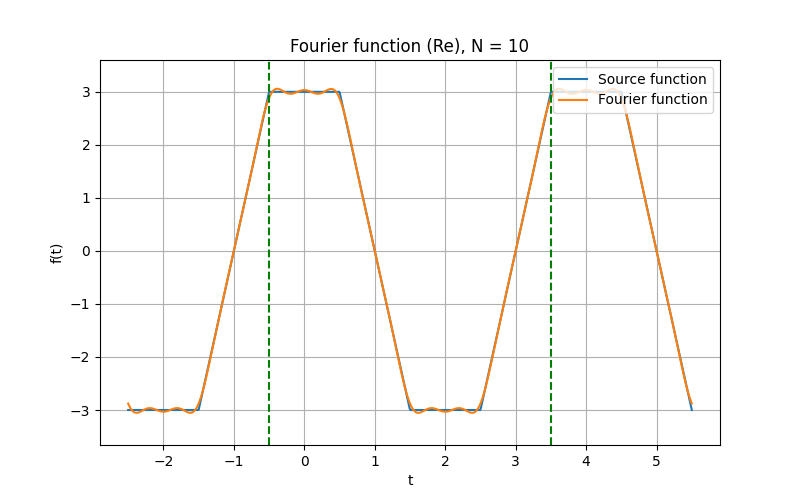
\includegraphics[width=0.49\textwidth]{media/plots/func_5_real_N_10.png}
    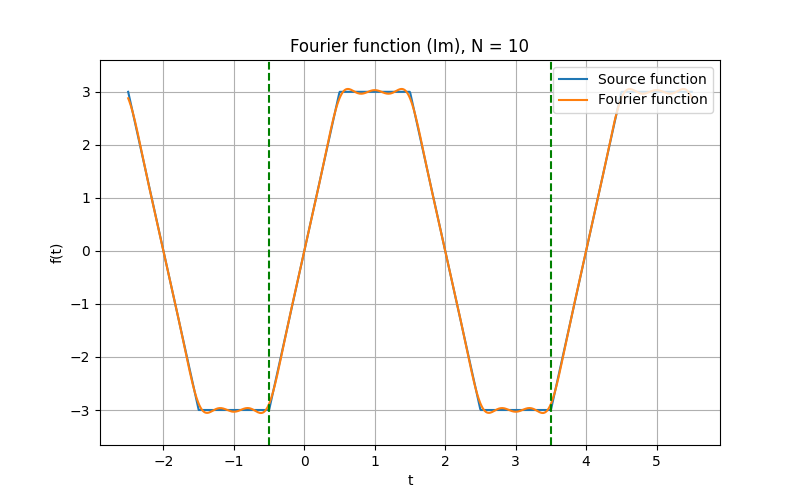
\includegraphics[width=0.49\textwidth]{media/plots/func_5_imag_N_10.png}
    \caption{График частичных сумм ряда Фурье для функции $f_5(t)$ ($N = 10$) (действительная и мнимая часть)}
    \label{fig:func_5_fourier_re_im_N_10}
\end{figure}

Тут так же заметно, что с увеличением значения $N$ график частичной суммы ряда Фурье все точнее приближает исходную функцию на выбранном промежутке. 
